\chapter{Data
  \label{chap:Data}}
%%% TABLE %%%%%%%%%%%%%%%%%%%%%%%%%%%%%%%%%%%%%%%%%%%%%%%%%%%%%%%%%%%%%%%%%%%%%
\begin{table}[ht]
\label{datasources}
\caption{Observational data sources used in this article}
\centering
\begin{tabular}{lrrrr}
\toprule
Instrument    & Central Wavelength & FWHM~$arcsec$ & Reference  \\
\midrule
AKARI/IRC & 9~$\mu$m     & 5.5$"$	     & \citep{irc07,ishihara10}  \\
AKARI/IRC & 18~$\mu$m	 & 5.7$"$       & \citep{irc07,ishihara10}   \\
AKARI/FIS & 65~$\mu$m    & 32$"$     & \citep{fis07,doi12} \\
AKARI/FIS & 90~$\mu$m    & 30$"$     & \citep{fis07,doi12} \\
AKARI/FIS & 140~$\mu$m	 & 41$"$     & \citep{fis07,doi12} \\
AKARI/FIS & 160~$\mu$m	 & 38$"$     & \citep{fis07,doi12}             \\ 
IRAS/IRIS & 12~$\mu$m    & 3.5$'$          & \citep{iris05}             \\
IRAS/IRIS & 25~$\mu$m    & 3.5$'$          & \citep{iris05}             \\
IRAS/IRIS & 60~$\mu$m    & 3.6$'$          & \citep{iris05}              \\
IRAS/IRIS & 100~$\mu$m   & 4.7$'$          & \citep{iris05}         \\
Planck/HFI & 345~$\mu$m & 4.7$'$ & \citep{hfi14viii} \\
Planck/HFI & 550~$\mu$m & 4.3$'$& \citep{hfi14viii} \\
\bottomrule
\end{tabular}
%\tabnote{}
\end{table}
%%%%%%%%%%%%%%%%%%%%%%%%%%%%%%%%%%%%%%%%%%%%%%%%%%%%%%%%%%%%%%%%%%%%%%%%%%%%%%%
\section{AKARI Space Telescope}
     The AKARI (Astro-F) infrared space telescope revealed an entire sky of infrared light, at wavelengths from the mid to far infrared, via two instruments \citep{akari07} the Infrared Camera (IRC)\citep{irc07} and the Far Infrared Surveyor (FIS)\citep{fis07}. Six all-sky maps were created, allowing for exploration into a great expanse of interstellar environments. The infrared sky had never before been revealed with such fine resolution at nearly unconstrained spatial coverage. In this work and many others, AKARI data has illuminated many patterns in the Milky Way. AKARI gave us a wealth of pointed imaging and spectroscopy observations, though for this study we have focused on the all-sky maps at 9, 18, 65, 90, 140, and 160~$\mu$m.

\subsection{AKARI/Infrared Camera}
     The Infrared Camera instrument on-board AKARI was designed to study the near to mid-infrared range, and was thus enabled with 7 observable wavebands. The world's only all-sky PAH-band survey, the IRC's 9~$\mu$m all-sky map demonstrates the abundance of the PAH bands carrier in the Milky Way \citep{ishihara10}. It is true that other instruments are capable of collecting emission from the PAH bands. However there is no other photometric instrument which has such a complete coverage of all of the major bands, at 6.2, 7.7, 8.6, and 11.2~$\mu$m \citep{onaka99,irc07}. In fact, the only other photometric survey with all-sky coverage at the MIR, the IRAS 12~$\mu$m band, did not collect any light from the 6.2, 7.7, or 8.6~$\mu$m bands, though it was somewhat sensitive to the 11.2~$\mu$m. WISE/Band 3 also has full-sky coverage, though its response functions are very similar to IRAS/12~$\mu$m. The Spitzer/IRAC bands are the only other photometric survey which dense coverage of the PAH bands. Though the wavelength coverage, sensitivity, and resolution of Spitzer/IRAC are extremely useful, the pixels are simply not available for most of the sky. Therefore, for the type of large spatial range study featured in this thesis, there is no other instrument suitable to investigate the PAH features than IRC. 
\begin{figure}[htbp]
\begin{center}
\label{allbands}
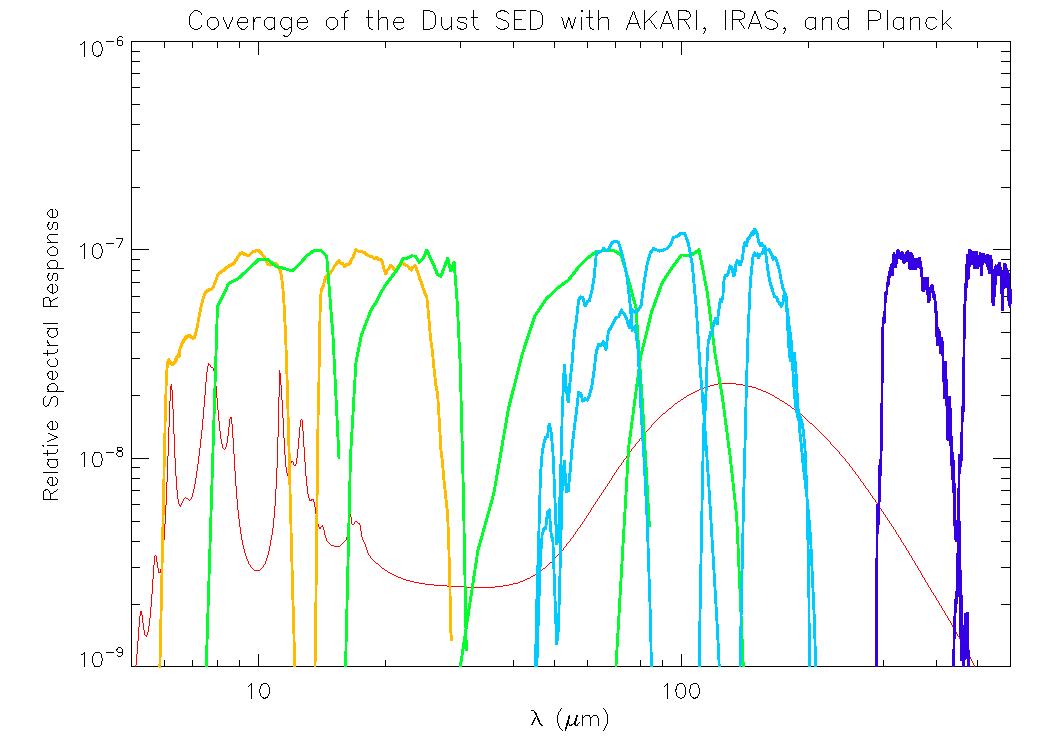
\includegraphics[width=150mm]{EPS/AKARI_rsr_thesis.pdf}
\caption{This figure describes our multi-wavelength analysis of the full vibrational dust SED.  The y-axis gives arbitrary relative response units. The x-axis shows the covered wavelength range in microns.The filter of each instrument's survey used in this study is plotted along with a sample dust mixture model SED computed by DustEM \citep{dustem11}. The AKARI/IRC 9 and 18~$\mu$m bands are shown in orange, FIS bands in turquoise, IRAS bands in green, and the Planck/HFI bands in purple. Most importantly, note the complete coverage of the major PAH/UIR bands 6.2, 7.7, and 8.6~$\mu$m by IRC \cite{ishihara10}. The IRAS 12~$\mu$m band's coverage starts at about 8~$\mu$m. The peak of the thermal emission curve is well covered by FIS.  The FIR tail of the thermal equilibrium emission curve is constrained by HFI.  To clarify, there is no significant contribution from AME at these wavelengths. These data are not intended to measure AME directly; only the corresponding information from thermal dust emission from AME regions is gathered.
 }
\end{center}
\end{figure}
%%%Let's put the filter response curves here
\begin{figure}[htbp]
\begin{center}
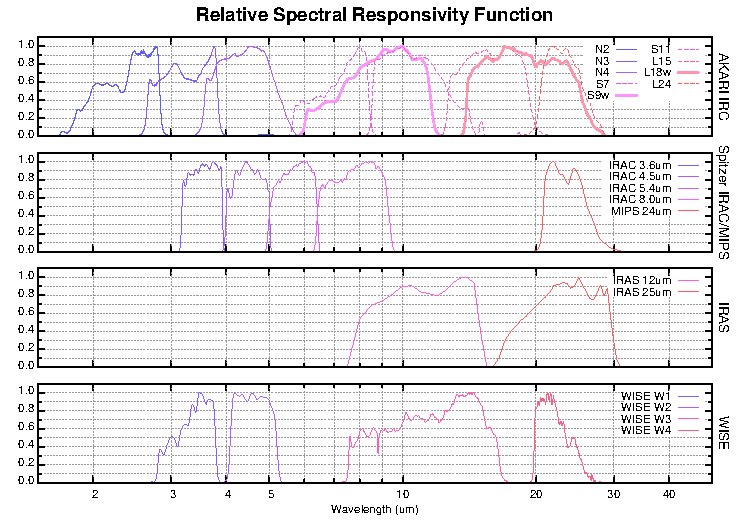
\includegraphics[width=150mm]{EPS/rsr.pdf}
\caption{
This image shows the filter response curves for the AKARI IRC bands vs. the bands from comparable instruments on-board the Spitzer, IRAS, and WISE infrared space telescopes. The most important thing to note is the coverage of the AKARI IRC 9~$\mu$m band vs. that of the IRAS~$\mu$m band and (and WISE band 3 which is very similar). The PAH / UIR bands cut-off just short of the IRAS 12~$\mu$m bands coverage, whereas the AKARI 9~$\mu$m survey spans most of the PAH bands, and the flux it observes is expected to be dominated by them. Though their central wavelengths are similar, we expect that the IRAS 12~$\mu$m and AKARI 9~$\mu$m bands contain very different information about the dust SED. While the Spitzer 8~$\mu$m band is similar, There is no other survey with such complete spectral and spatial coverage of the PAH bands. AKARI is a critical tool for this type of PAH investigation spanning such a large number of ROIs.
 }
\label{rsr}
\end{center}
\end{figure}
\subsection{AKARI/Far Infrared Surveyor}
     The Far Infrared Surveyor (FIS) gives us photometric data around the peak of the typical dust SED. FIS was equipped with four wavebands: two narrow bands centered at 65~$\mu$m and at 160~$\mu$m, and two wide bands at 90~$\mu$m and at 140~$\mu$m. An all-sky scanning survey was carried out at each band \citep{doi12}, and the processed maps have been recently released at the time of this writing. Figure \ref{fig:FIS} shows the all-sky map at 140~$\mu$m produced by FIS.
%%%\citep{doi14}%%%%
\begin{figure}[!htb]
\begin{center}
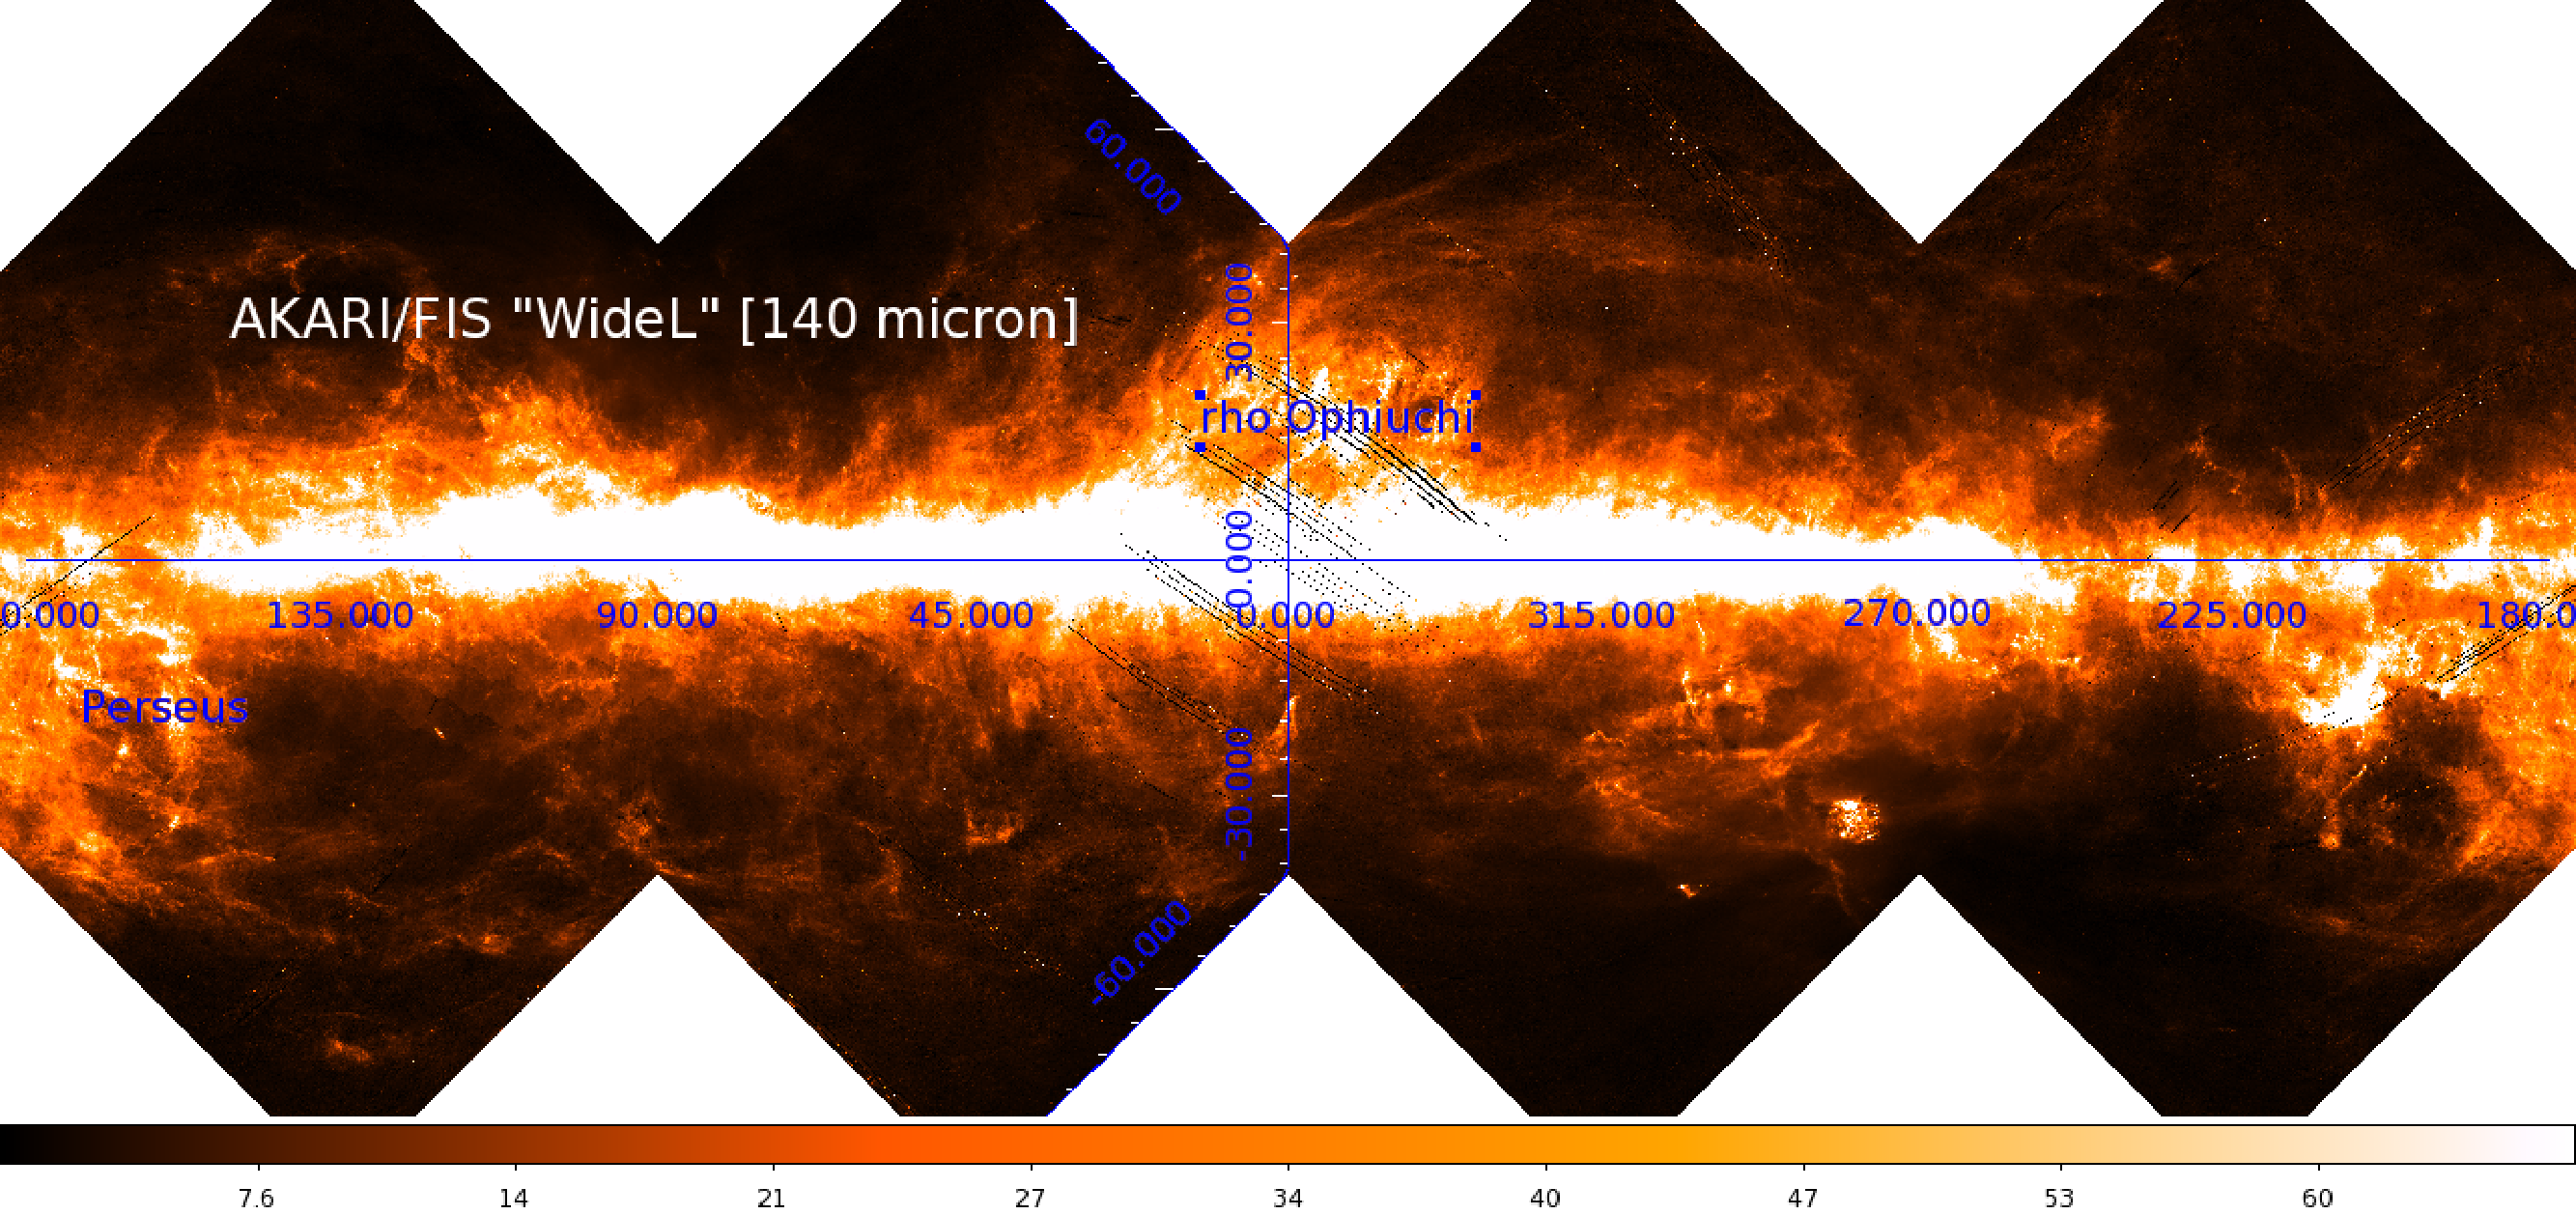
\includegraphics[width=170mm]{EPS/im_akari140.pdf}
\caption{This is the Milky Way according to the AKARI/FIS 140~$\mu$m data. The two most prominent AME regions, Perseus and $\rho$~Ophiuchi are labelled in blue. The coordinates are Galactic. This is the highest resolution data available in the FIR wavelengths, with such wide spatial coverage. The stripe errors which affect mostly the regions around Ophiuchi are visible. This map is the HEALPix 1.7arcmin/pixel version (much lower resolution than the $~$30~arcsec original all-sky maps). The colorbar is in MJy/sr.}
\label{fig:FIS}
\end{center}
\end{figure}



The narrow bands have a higher noise-level compared to the wide bands. However the absolute photometric uncertainty per pixel has yet to be evaluated. The main point is that FIS samples a critical part of the dust SED not sampled by IRAS, and at galactic latitudes beyond the reach of the Spitzer Space Telescope \citep{spitzer04}.

\section{Planck High Frequency Instrument (HFI)}
     The latest and most accurate CMB surveys are created by the Planck Space Observatory (Planck), with its Low Frequency Instrument (LFI)  ranging from 30 to 70~GHz \citep{lfi14ii}, tracing the peak CMB and a large portion of the galactic foreground, and its High Frequency Instrument (HFI) spanning 100 to 857~GHz \citep{hfi14viii}, which traces much of the galaxy’s thermal emission.
     While the largest-scale patterns of the sky, those of the CMB have been studied carefully by both the LFI and HFI, the HFI instrument has talent for ISM research as well. The far infrared thermal emission tail of the dust spectral energy distribution can be constrained by the HFI’s photometric bands. This study uses the all surveys in the 857~GHz (345~$\mu$m) and 545~GHz (550~$\mu$m) bands, respectively, for their unique coverage of the post-peak dust SED complemented the SED-peak constraints provided by AKARI/FIS. These data points are critical for regions-of-interest that were spatially beyond the reach of Planck’s partner sister observatory, Herschel. Without Planck data we cannot strongly constrain the temperature and column density of interstellar dust.
\section{IRAS}
     Data from the Infrared Astronomical Satellite \citep{iras84} all-sky surveys are used to supplement the similarly-centred AKARI photometric bands. Including IRAS data offers a more dense sampling of the dust SED in regions where Spitzer or Herschel data are simply non-existent.T
     The IRAS 12~$\mu$m band is similar to the AKARI 9~$\mu$m band in terms of the sky coverage, central wavelength, and especially in that both surveys are heavily dominated by zodiacal light. The model of zodiacal dust emission (zody) by \cite{mrr13} utilized for the Improved Reprocessing of the IRAS Surveys (IRIS) \citep{iris05} is an important benchmark for the zody-subtraction from the AKARI/IRC surveys.
\section{All-sky Data Handling}
\subsection{Data Extraction}
       The data extraction process uses primarily standard routines, relying on the Interactive Data Language (IDL) platform. The framework for the data processing outlined below essentially follows the structure prepared by Fr\'ed\'eric Galliano for the Herschel-Planck School 2013 (http://ecole-doctorale.obspm.fr/-Program-). The course utilized example IDL routines and Herschel data as a curriculum to teach basic processing and dust SED fitting of an extended object. In this study, those examples are adapted and expanded to handle AKARI data. A color-correction step is added which is based on the DustEM IDL wrapper code \citep{dustem11}. The final step of Galliano’s example is to apply a custom full dust SED fitting routine. However dust model templates for this step have not yet been created for the AKARI data. The average SEDs for each region are instead piped to the DustEM code. The results between DustEM and Galliano’s model will be compared in a future work.
\subsection{Target Selection}
%%%***Include Table***%%%
     Regions of interest (ROI) were chosen based on their relevance to AME research. In general, we follow the work of PCXV. In this recent study of the AME in the dense galactic ISM, candidate “spinning dust regions” were selected using a 2 to 3 degree wide selection criteria. 2 degree-wide apertures which showed excess emission after subtraction of synchrotron, free-free, CMB, and thermal dust emission, were listed as candidates. The Planck team then conducted a multi-wavelength SED modelling of each region at all Planck/LFI and HFI frequencies, to determine the likelihood that its excess is explained by spinning dust. For this purpose they employed the ``SPDUST” model, developed by \cite{ali-hamoud09}. Some targets were shown to be extremely likely spinning-dust regions, such as $\rho$ Ophiuchi with a confidence level of $~30\sigma$. Other regions were dismissed as spinning dust targets by PCXV after spectral modelling, as in the case of the Orion Nebula whose SED was well explained by free-free emission. \par    
     The original intention of this thesis was to look at the fine-scale spatial variations of the dust SED, primarily at the MIR wavelengths relevant to PAHs/very small dust, in $\rho$ Ophiuchi and Perseus. We intended to compare works such as \cite{tibbs11} which focused on Spitzer data, with data from AKARI. This is why we first do a pixel-by-pixel analysis of each ROI. However the strategy was modified later on when the PCXV results were released, identifying a large number of candidate AME regions. We now focus on the average SED of each ROI for the purpose of understanding the AME. This method may also be generally useful as a study of the typical AKARI+IRAS+HFI SED across a large number of galactic clouds.
     This thesis first aims to complement the PCXV analysis of AME regions by contributing dust SED analysis using unique compilation of photometric data, i.e. the AKARI/IRC 9~$\mu$m survey’s coverage of the PAH/UIR bands. We have selected ROIs having an array of AME significance values. Regions such as Orion, described as “non spinning dust regions” in PCXV are used as a control against regions suspected to exhibit spinning dust.

\subsection{HEALPiX maps}
     In the case of the FIS, HFI, and IRAS bands, ROI’s are cut-out out from all-sky .FITS files, structured according to the Hierarchical Equal Area isoLatitude Pixelization (HEALPix) scheme \citep{healpix05}, a standard data format conceived to handle very large data sets, and originally used for the WISE surveys. It works very efficiently as a framework for all-sky maps processing, especially in the case of degrading to a lower pixel resolution. There are also many standard routines available for processing HEALPix-formatted data. 
     In this work, the particular advantage that ROI cut-outs can be very easily created from a pre-compiled HEALPix array was desired. The ROIs are extracted using a “cookie-cutter” routine with the very recallable name of GNOMDRIZZ, part of the publicly available DRIZZLIB IDL package.  Cut-outs for each of the FIS, HFI, and IRAS bands are extracted easily, without the need to mosaic a series of tile images.  The HEALPix framework also defines common resolution tiers, and the “Resolution Level 11”, or NSIDE 2048 is chosen for the processing described here. This is the highest common resolution map offered across the three instruments, having a pixel scale of 1.7$'$. During the GNOMDRIZZ extraction, we keep the 1.7$'$ pixel scale for the tangential projection of each map according to the galactic coordinate system. We believe the 1.7$'$ pixel scale is in good proportion to the 857~GHz band’s beam-size of 4.7$'$.
\subsection{Region extraction}
     In order to keep a standard reproducible method for our data processing, all of the ROIs are handled in the same way. The NSIDE 2048 native pixel scale of 1.7$'$ is kept, and a pixel dimension of 47 is chosen so that each ROI cut-out is (80$')^2$ . Given the typical size of the primary ROI class (HII regions falling in an ``AME zone", usually around 0.5\degree wide), an 80$'$ square map should be appropriately sized to contain both the ROI and a sufficient number of background pixels. Figure \ref{fig:PCXVresmap} shows the residual map from PCXV from which their AME ROIs were selected.
\begin{figure}[htb!]
\begin{center}
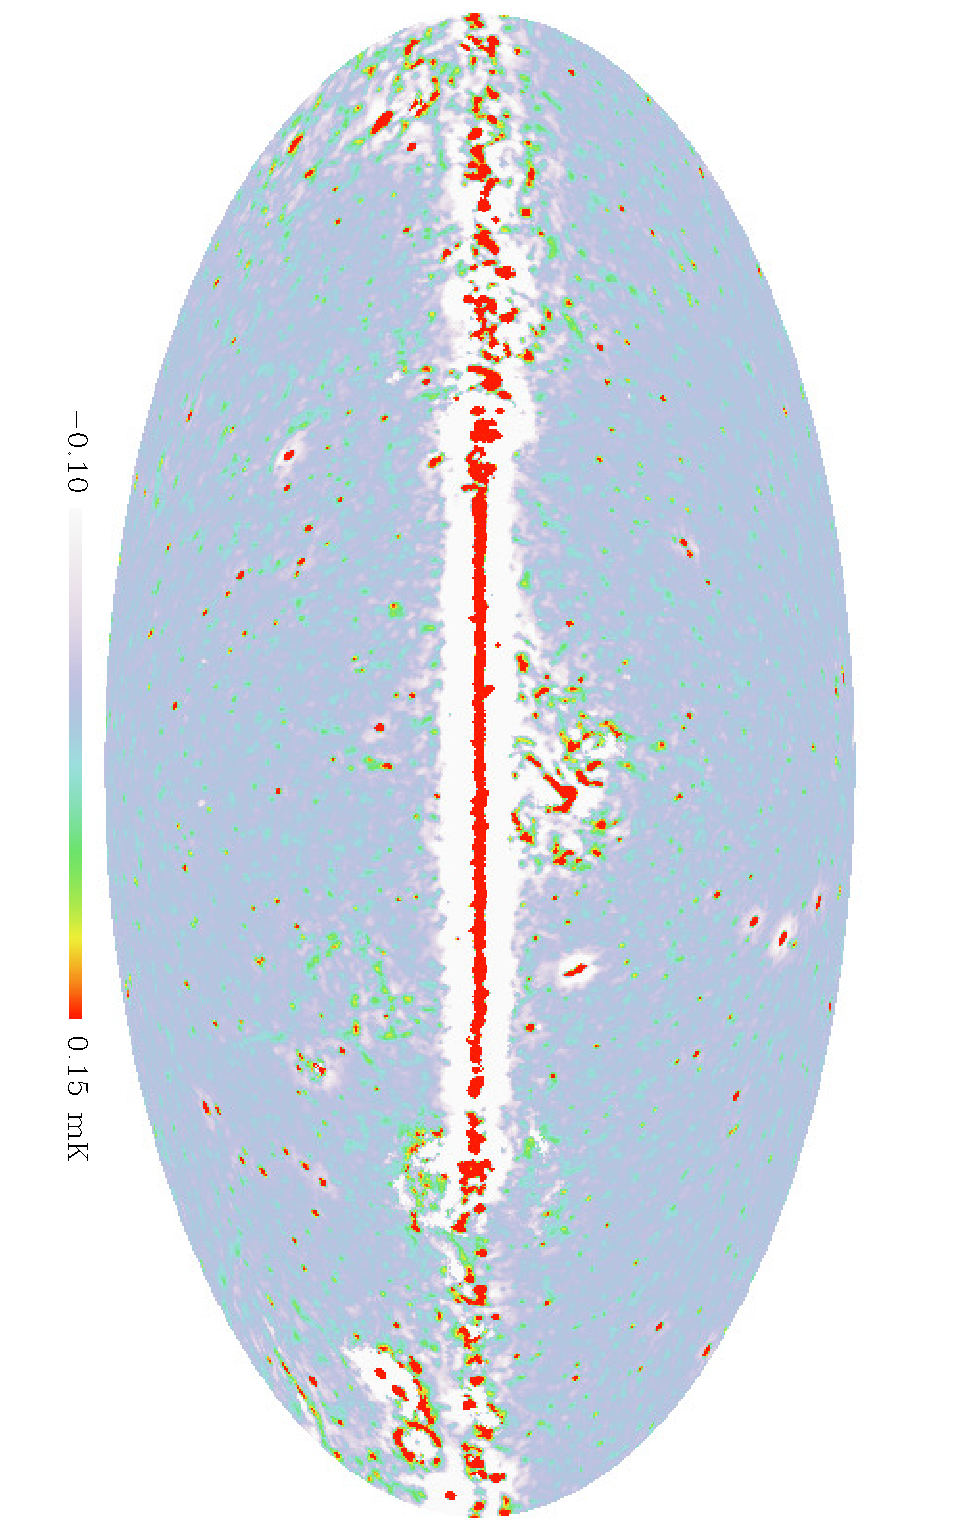
\includegraphics[width=80mm, angle=90]{EPS/planckXV_fig1.pdf}
\label{PCXVmap}
\caption{This map illuminates the suspected AME regions across the entire sky. From \cite{planckXV}, the authors subtracted models of free-free, synchrotron, and thermal dust emission from the LFI 28.4~GHz map to produce this ``residual map" which is a general tracer of  the AME. Many of the bright red regions in this image are believed to exhibit spinning dust emission.}
\label{fig:PCXVresmap}
\end{center}
\end{figure}

\subsection{Background Subtraction}
     Background subtraction is always an interesting problem and especially for these types of near-by ISM complexes having non-trivial structures. The possibility of subtracting the target emission itself along with the ``background” is a common risk. For very bright regions where the only significant source of background emission is the zody, we believe that a simple flat background subtraction is suitable. A fitted-plane background subtraction may be appropriate for regions near to the ecliptic plane, such as $\rho$ Ophiuchi. For other, faint regions, or those within the galactic plane where chances of confusion with other targets is higher, a more careful approach is ultimately desired. In the case of FIS data, the smooth component of the zody has already been subtracted. The IRAS/IRIS data has already been zody-subtracted. 
     In this first study however, we have adopted a standard way to subtract the background. We subtract a flat-average background from each ROI using a commonly available routine ``BACKSUB”, in the Buie Astronomy IDL Library.Other background methods may be more or less effective, depending on the region, however we have chosen to keep a very standard procedure for this study. Later studies will utilize a more sophisticated subtraction approach, and compare the results for various methods (i.e. flat-mean subtraction vs. 2D polynomial subtraction.
     Following the background-subtraction, the arrays for each region are ``zoomed-in”. We decrease the image size to include only a 30~$'$ square patch around the ROI’s center coordinates. This width is chosen as a suitable average size range for each region. A larger window leaves us over-sampling background positions for some narrower ROIs, while a smaller window may be offset from the cloud’s structure. In the PCXV analysis which we initially followed, a 1$\degree$-radius circular aperture was used for sampling. However their maps were also subject to a much coarser smoothing, using a 1$\degree$ Gaussian beam. Our study is not directly comparing infrared data to the low resolution microwave data, thus this smoothing is not needed. However in a later analysis, we would like compare our present study with the same analysis done according to the PCXV smoothing and aperture size.
\subsection{Pixel masking}
%%Insert a figure showing the masking of the saturated pixels of Orion %%%
     Upon the final SED extracting and modified blackbody fitting, any pixel which is masked at any of the sampled wavebands, is masked for the entire fitting. The final mask is a super-position of all of the individual wavebands’ masks. In other words, only pixels which are unmasked for all wavebands are used. 
     Pixels having negative values after the background subtraction are masked from the analysis. In this way, we are assuming that those pixels were too close to the ``true background level”. Rather than adjusting the background level to avoid negative values, we mask these pixels from the data processing and SED fitting. 
     Due do this super-positioning of masks, the background mask size and shape is more sensitive to the IRC data. This is because there is a tendency for the bright regions in the AKARI/IRC data to be more compact than the same regions as observed by AKARI/FIS. Thus the final sampled portion of each ROI is biased towards the apparent region size seen in the AKARI 9 and 18~$\mu$m all-sky data.          
     Pixels that already have zero or ``not-a-number” values applied to them during the original data reduction remain masked in this study. They are not filled in with data from alternate surveys. In any case, this masking is not a common issue; usually it is a result of saturated pixels covering very bright targets. The center of Orion (M42) is a good example, in the FIS data. $\rho$~Ophiuchi contains some missing ``stripes” due to the AKARI’s pointing being changed to accommodate individual observation requests during the all-sky scanning of that region. Neither of these issues (over-saturation or missing stripes) have been relevant for the Planck HFI data. 
\subsection{Resolution Degrading}
     All of the data in this analysis was smoothed according to a larger beam size, because of one disadvantage incorporating the Planck HFI data. The beam size of the 545~GHz band is roughly 4.7$'$. This means the native resolution AKARI data is not comparable to the Planck data, or IRIS data, in a pixel-by-pixel manner. Despite the disadvantage, Planck’s extended FIR wavelength coverage is critical to make a trustable SED fitting. In order to find a compromise, we degrade the resolution of AKARI IRC and FIS data to that of the Planck HFI beam. While it is perhaps superficially discouraging to degrade visually appealing high resolution data, in this case the SED coverage is of a higher priority. Even HFI’s larger beam size is fine enough for our purposes this type of large-scale study.
     All of our data is convolved with the largest beam of the Planck HFI 545~GHz waveband, having a resolution of about 4.7$’$. The beam’s shape is sufficiently elliptical that we have acquired the publicly available Planck Legacy Archive HEALPix file containing the HFI-team-provided PSF, rather than simply convolving with a circular Gaussian beam. This allows us to at least keep the resolution of our final data set at 4.7$’$. As we were initially interested in smaller-scale variations (before expanding the number of ROIs to include all 98 PCXV regions). We felt that convolving with a larger artificial circular Gaussian PSF would have unnecessarily constrained our study. For future work we may experiment with a much coarser smoothing. 
     We are interested not only in the average SED of each ROI, but also, as much as possible, we want to begin to understand the structural variations within the region. The actual convolution processing is handled by the IDL routine \textit{DO\_THE\_CONVOLUTION} which is publicly available and developed by \cite{aniano11}.
     We have not created kernels between the AKARI data and the Planck data, nor between the AKARI/IRC and AKARI/FIS.  The Planck beam is sufficiently large compared to the respective beam sizes of the AKARI instruments that a kernel was not needed. For future purposes, it will be useful to create convolution kernels between the IRC and FIS beams, such that we can explore the structural detail in these surveys side by side.
\subsection{Regridding}
     A ``regridding” step is included so that the positions of the cut-outs made from HEALPix maps (as in the case of AKARI FIS) can be aligned with cut-outs which are made via mosaicking the original survey tiles (as in the case of AKARI IRC). All of the HEALPix maps are already aligned to the same grid during the drizzling process, which creates a rectangular FITS file from a HEALPix map. At that time a galactic World Coordinate System (WCS) and identical pixel scale and image dimensions are chosen. However images not created using the HEALPix standard routines need to be re-gridded so that they match, pixel-by-pixel, the positions of the HEALPix-generated cut-outs.
\subsection{Color Correction and Modified Blackbody Fitting}
     One fundamental issue in photometric studies is that such bandpasses are not evenly sensitive at all wavelengths which they cover. Therefore, there is some deviation between the emission which they observe and what is actually being produced. We may never be able to infer perfectly what the actual source's emission characteristics are. Fortunately, we can get a good approximation of the sources SED if we first know what type of emission it is most likely producing. Then we may use the observed emission to scale a template SED model. In the case of thermal dust emission in the FIR, we expect the continuum emission to basically take the shape of a blackbody, though with a correction applied to the emissivity. The form of the equation for such emission was given in Chapter 1:
\begin{equation*}
\tag{1.3.3}
I_d(\nu) \propto \nu{}^{\beta{}_d}B_\nu{}(T_d)
\end{equation*}
     We first fit the non-color-corrected data with the above equation, fitting $T$ to each one (with $\beta$ fixed at 2.0), as well as an ``amplitude" (explained more carefully in Chapter 3). With this initial fitted model spectra, we convolve with response functions of the bands greater than 65~$\mu$m to obtain the color correction factors. The color-correction routine is borrowed from the DustEM IDL wrapper code \citep{dustem11,dustem13}.
     The color correction factors are then applied to the observed intensities of their corresponding bands. Finally, the modified blackbody fitting is run again in order to obtain the $T$ and amplitude of the expected FIR SED at each unmasked pixel.
     Using the fitted values, a mean average of the temperature, and the color-corrected intensity at each wavelength, is taken across the unmasked pixels. These average values, calculated for each of the 98 ROIs from PCXV are used in the plots against AME parameters (from the same paper) in Chapter 3.
%\subsection{Black-hole Sample Return Mission Results}
%Unfortunately the entire mission apparatus (including the human components) was spaghettified exactly as predicted. However we have no way of knowing if this really happened or not, as no information was retrieved from the event. There was one slight anomalous increase in the X-ray flux from the AGN for a moment of time that we cannot quantify. We can only conclude that science is a lot of fun, and we would gladly do it all over again.
%\section{High Resolution Case Study: Perseus and $\rho$ Ophiuchi}
%In addition to the large scale data extracted across all regions presented in PCXV, we examined two very heavily studied AME candidates: the Perseus Molecular Cloud Complex and $\rho$ Ophiuchi. We examine these two regions spatially in the IRC 9 and 18~$\mu$m data at their native resolution vs. contours derived from the Planck 2014 Release "low-frequency diffuse emission" map.
